% !TEX program = xelatex
\documentclass[a4paper,10pt]{article}
\usepackage[margin=2.05cm]{geometry}
\usepackage{fontspec}
\usepackage{graphicx}
\usepackage{booktabs}
\usepackage{tabularx}
\usepackage{array}
\usepackage{amsmath}
\usepackage{microtype}
\usepackage{xcolor}
\usepackage{hyperref}
\usepackage{caption}
\usepackage{subcaption}
\usepackage{float}
\usepackage[numbers,sort&compress]{natbib}
\graphicspath{{figures/}}
% Generated by scripts/generate_dataset_figures.py.
\newcommand{\DatasetSceneCount}{10}
\newcommand{\DatasetTiffCount}{60}
\newcommand{\DatasetUsablePatchCount}{1800}
\newcommand{\DatasetPrivacyExcludedCount}{25}
\newcommand{\DatasetFixedTrainCount}{1141}
\newcommand{\DatasetFixedValidationCount}{270}
\newcommand{\DatasetFixedTestCount}{389}
\newcommand{\DatasetTaskFileCount}{14400}
\newcommand{\DatasetRawFileCount}{1281}
\newcommand{\DatasetSourcePositionCount}{140}
\newcommand{\DatasetRgbFrameCount}{581}
\newcommand{\DatasetSwirFrameCount}{700}
\newcommand{\DatasetPoseEdgeCount}{591}
\newcommand{\DatasetOutputScale}{3.2}
\newcommand{\DatasetAcquisitionDateMin}{2025-04-29}
\newcommand{\DatasetAcquisitionDateMax}{2025-11-28}
\newcommand{\DatasetCoverageMin}{0.712}
\newcommand{\DatasetCoverageMax}{0.902}
\newcommand{\DatasetCoverageMean}{0.841}
\newcommand{\DatasetBuildSecondsMin}{48.6}
\newcommand{\DatasetBuildSecondsMax}{908.1}
\newcommand{\DatasetRedactedSceneUsablePatchCount}{131}
\newcommand{\RegHoldoutMinPx}{3.56}
\newcommand{\RegHoldoutMedianPx}{5.73}
\newcommand{\RegHoldoutMeanPx}{6.06}
\newcommand{\RegHoldoutMaxPx}{9.23}
\newcommand{\RegCornerMinPx}{1.56}
\newcommand{\RegCornerMedianPx}{3.03}
\newcommand{\RegCornerMeanPx}{5.70}
\newcommand{\RegCornerMaxPx}{27.78}
\newcommand{\RegCornerWorstScene}{C5}
\newcommand{\RegCornerRunnerUpPx}{8.60}
\newcommand{\RegCornerOutlierRatio}{3.2}
\newcommand{\RegCornerOtherMeanPx}{3.24}
\newcommand{\RegCornerGateMinPx}{25.6}
\newcommand{\RegCornerGateMaxPx}{76.3}
\newcommand{\IntraSwirMinPx}{3.19}
\newcommand{\IntraSwirMeanPx}{4.74}
\newcommand{\IntraSwirMaxPx}{6.25}
\newcommand{\IntraSwirGatePx}{8}

% 主结果宏：数值来自 outputs/summary_v2_20261005/main_table.csv（十地点等权）
% 核对日期 2026-10-15；口径：单种子 11、暂定共同支持、固定末步检查点
% 中英文共用；宏名只含字母。数值由 scripts/qa_manuscripts.py 对源表核验。
\newcommand{\SupportPixelCount}{88861466}
\newcommand{\QualifiedWindowCount}{5893}
\newcommand{\LpipsRectCount}{1541}
\newcommand{\TrainRunCount}{30}
\newcommand{\SensitivityRecordCount}{330}
\newcommand{\GeneralizationGap}{11.78}

% 主表 PSNR（十地点等权）
\newcommand{\PsnrLinearFive}{14.1083}
\newcommand{\PsnrRestormerFive}{13.7961}
\newcommand{\PsnrUnetFive}{12.8229}
\newcommand{\PsnrTfdFive}{12.8283}
\newcommand{\PsnrPixFive}{12.5993}
\newcommand{\PsnrPixBOne}{12.9972}
\newcommand{\PsnrPixBOneTwoFour}{13.0413}
\newcommand{\PsnrChannelFive}{10.6005}

% SSIM
\newcommand{\SsimRestormerFive}{0.5612}
\newcommand{\SsimLinearFive}{0.5589}
\newcommand{\SsimLinearBOne}{0.5743}
\newcommand{\SsimPixBOne}{0.5014}

% LPIPS
\newcommand{\LpipsLinearFive}{0.4606}
\newcommand{\LpipsRestormerFive}{0.5016}

% DeltaE00
\newcommand{\DeltaELinearFive}{19.7135}
\newcommand{\DeltaERestormerFive}{20.5228}

% 跨地点泛化
\newcommand{\SeenPsnr}{25.37}
\newcommand{\HeldoutPsnr}{13.59}
\newcommand{\SeenWindowCount}{89}
\newcommand{\HeldoutWindowCount}{43}

% 聚合口径敏感性（像素汇总）
\newcommand{\PooledPsnrLinear}{13.3762}
\newcommand{\PooledPsnrRestormer}{13.5359}

\hypersetup{colorlinks=true,linkcolor=black,citecolor=black,urlcolor=blue}
\setlength{\parindent}{0pt}
\setlength{\parskip}{0.45em}
\captionsetup{font=small,labelfont=bf}

\newcommand{\dE}{\ensuremath{\Delta E_{00}}}

\title{\textbf{A Scene-Level Paired RGB and Five-Band Short-Wave Infrared Dataset for Cross-Spectral Image Synthesis}}
\author{Hu Du$^{1,2,*}$, Xiao Liu$^{2,3,\dagger}$, Lili Du$^{2,3}$, and Hu Cui$^{2}$\\[0.35em]
\small $^{1}$University of Science and Technology of China, Hefei 230026, China\\
\small $^{2}$Hefei Institutes of Physical Science, Chinese Academy of Sciences, Hefei 230031, China\\
\small $^{3}$Key Laboratory of Optical Calibration and Characterization,\\
\small Anhui Institute of Optics and Fine Mechanics, Chinese Academy of Sciences, Hefei 230031, China\\[0.25em]
\small $^{*}$Correspondence: \href{mailto:2542497213@qq.com}{2542497213@qq.com} (H.D.); $^{\dagger}$\href{mailto:liux@aiofm.ac.cn}{liux@aiofm.ac.cn} (X.L.)\\
\small ORCID (H.D.): \href{https://orcid.org/0009-0006-1742-2455}{0009-0006-1742-2455}}
\date{}

\begin{document}\maketitle
\begin{abstract}Paired RGB and short-wave infrared (SWIR) imagery requires explicit spectral definitions, spatial correspondence and evaluation units to support reproducible reuse. M-SWIR-RGB contains ten scene mosaics from ten distinct physical sites. Its archive comprises 1,281 raw files (581 RGB and 700 SWIR) from 140 acquisition positions; the mosaics use 840 selected frames (140 RGB and 700 SWIR). Each site provides RGB and five nominal SWIR sub-bands, yielding 60 eight-bit TIFF files. The five bands are acquired sequentially and are not radiometrically calibrated. We document source identity, geometric transforms, radiometric processing and privacy exclusions. An exploratory site-disjoint five-fold benchmark compares four models and two non-neural references on shared provisional support, using 30 training runs with seed 11 and 330 misalignment-sensitivity records. The best learned model by site-equal PSNR, Restormer, is 0.31\,dB below a linear reference fitted on training sites; the paired confidence interval crosses zero, and pixel pooling reverses the ordering. In the pix2pix ablation, five bands improve colour discrepancy but reduce SSIM relative to B1, indicating a metric trade-off rather than a uniform gain. Registration is characterized by automatic pipeline diagnostics and controlled-misalignment responses, neither of which independently measures registration accuracy. The contribution is a traceable multiband resource and a recomputable site-disjoint protocol, with no new model.\end{abstract}
\section{Background and summary}
Short-wave infrared (SWIR) imaging provides information that is difficult to obtain in the visible. First, the SWIR reflectance contrasts of typical ground materials (vegetation, dry grass, bare soil, water, pavement) are inconsistent with their visible colour differences, so materials that are hard to separate in RGB can be distinguishable in SWIR \cite{song2024,sivaprakasam2023}. Second, SWIR radiation suffers weaker scattering attenuation by fog and aerosols than visible light and retains imaging capability under low illumination and adverse weather \cite{narasimhan2002,bijelic2020fog,bessonov2025}; defogging studies that jointly model SWIR and visible transmittance exploit the same complementarity \cite{duan2025}. With progress in InGaAs and quantum-dot detector technology, SWIR imaging is moving from dedicated remote sensing towards ground-level, automotive and UAV platforms \cite{rogalski2003,yu2024,bessonov2025}.
\begin{figure}[htbp]\centering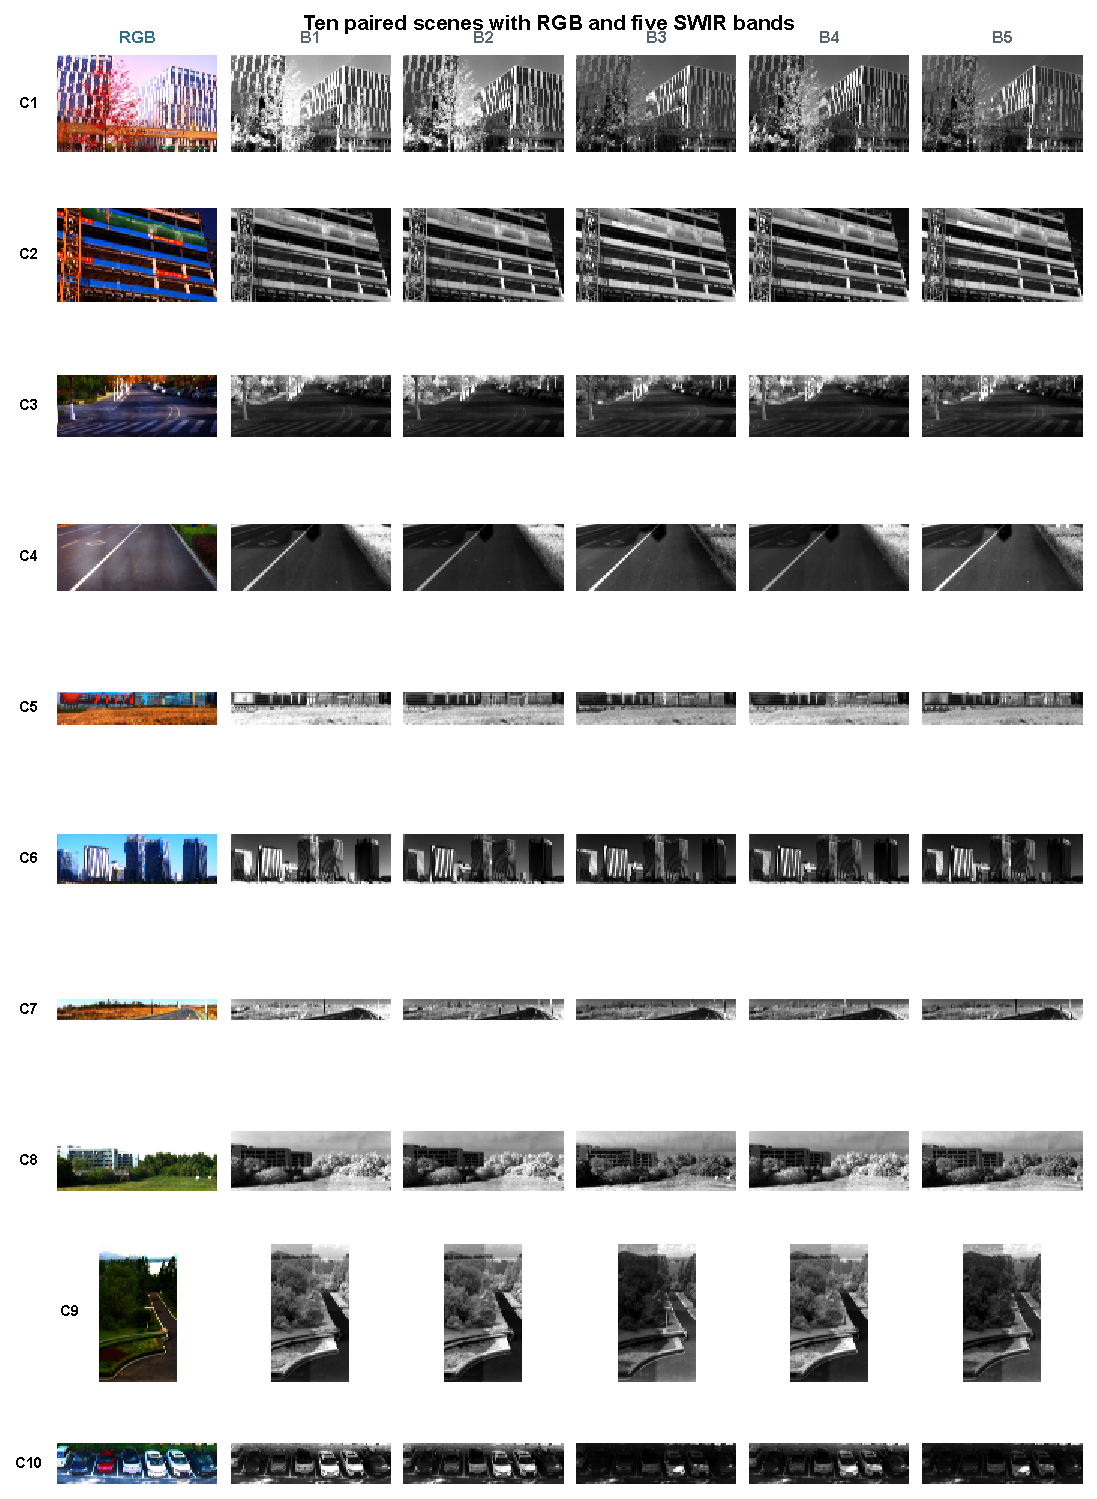
\includegraphics[width=\textwidth]{fig1_scene_modality_overview.pdf}\caption{Six-modality mosaic overview.}\label{fig:overview}
\vspace{1pt}{\footnotesize\noindent The display-only global percentile stretch is not used in evaluation; this plate does not establish local registration accuracy.\par}\end{figure}
The deep-learning exploitation of these capabilities mainly follows the cross-spectral generation route: reconstructing visible appearance from SWIR or near-infrared inputs (colorization) or synthesizing infrared bands from visible images, for interpretable visualization of infrared imagery and cross-modal tasks, with methods evolving from optimization and adversarial networks to diffusion models \cite{levin2004colorization,zhang2016colorful,chen2025,borstelmann2024,chen2026threeband}. Like visible--infrared segmentation, detection, matching and fusion tasks, such supervised methods rely on pixel-level aligned paired resources \cite{isola2017,ha2017,hwang2015,jia2021,razakarivony2016,liu2023segmif}; multi-band datasets containing a SWIR channel have also begun to appear in recent years \cite{liu2025triband}. The alignment quality and spectral coverage of paired data influence the correspondences a model can learn and the interpretation of evaluation results.
Existing RGB--SWIR resources differ in spectral coverage, pairing and evaluation units (Table~\ref{tab:related}). Spectral dimension: RASMD provides one broadband SWIR channel (1000--1700\,nm) \cite{jin2026}, and the recent tri-band detection dataset also contains a single broadband SWIR channel \cite{liu2025triband}; these resources do not resolve multiple SWIR sub-bands. DeepSWIR synthesizes SWIR from coarse-resolution satellite multisensor bands \cite{rout2019}, whereas the EPFL resource covers near-infrared rather than SWIR \cite{brown2011}. The earlier same-platform work also acquired RGB and five SWIR sub-bands; B1/B2/B4 was a model input configuration \cite{chen2026threeband,chen2026thesis}. Differences from that resource require disclosure of image overlap, site identities and evaluation protocols. Geometric dimension: separately acquired views require post-hoc registration, as in RASMD's SIFT homography with RANSAC \cite{jin2026} and AVIID's separate aerial acquisitions \cite{aviid2023}. Such pairing can retain residual mismatch, a difficulty also addressed by joint registration and fusion methods \cite{tang2022superfusion}. Protocol dimension: the same-platform thesis reports a random 4:1 train/test split \cite{chen2026thesis}; its related journal paper reports a macro-scene 80/10/10 split \cite{chen2026threeband}. Without a mapping between those macro-scenes and the physical sites in this manuscript, neither split can be treated as equivalent to the present site-disjoint protocol. Correlated views or patches also require care when interpreting generalization \cite{roberts2017}. Explicit source provenance, support definitions and evaluation units help reusers judge these differences \cite{gebru2021,wilkinson2016}. M-SWIR-RGB therefore provides multiple SWIR sub-bands together with a traceable site-disjoint colorization protocol that can be recomputed on common support.
\begin{table}[htbp]
\centering
\caption{Structural comparison with related paired resources.}\label{tab:related}
\vspace{1pt}{\footnotesize\noindent Entries for other resources are taken from their published descriptions; ``n.r.'' means not reported in the cited work. Macro-scenes in earlier work have not been mapped to the physical sites in this manuscript.\par}
\small
\begin{tabularx}{\textwidth}{@{}p{0.13\textwidth}p{0.17\textwidth}p{0.20\textwidth}p{0.20\textwidth}X@{}}
\toprule
Resource & Domain & Spectral content & Pairing mechanism & Organization and splits\\
\midrule
RASMD \cite{jin2026} & Driving, urban/suburban, sunny, cloudy, rain, snow & RGB plus one broadband SWIR channel (1000--1700\,nm) & Two separate cameras, post-hoc SIFT homography with RANSAC & $10^5$ RGB/SWIR image pairs; task-specific subsets\\
AVIID \cite{aviid2023} & Aerial, vehicle targets & Visible and infrared patch pairs & Separate aerial acquisitions & 993, 1090 and 1280 pairs at $434\times434$ or $512\times512$; patch-level\\
DeepSWIR \cite{rout2019} & Satellite multisensor & SWIR band synthesized from green, red, NIR and coarse SWIR & Cross-sensor co-registration at 5 and 24\,m GSD & n.r.\\
Same-platform thesis \cite{chen2026thesis} & Ground scenes, four categories & RGB plus five SWIR sub-bands; model inputs B1/B2/B4 & Common-aperture platform, mosaic then sliding window & 4000 patch pairs; reported random 4:1 train/test split\\
Same-platform journal paper \cite{chen2026threeband} & Ground scenes & RGB plus five SWIR sub-bands; model inputs B1/B2/B4 & Common-aperture platform, mosaic then sliding window & About 4000 pairs; reported macro-scene 80/10/10 split, augmentation for training only\\
M-SWIR-RGB (this manuscript) & Ground scenes, ten distinct physical sites & RGB plus five SWIR sub-bands (nominal passbands; response not measured) & Common-aperture dichroic platform; feature-based pose graph per scene & \DatasetSceneCount{} scenes; \QualifiedWindowCount{} candidate windows; site-disjoint train/validation/test\\
\bottomrule
\end{tabularx}
\end{table}
M-SWIR-RGB combines three design choices. Spectral: the five narrow SWIR bands (B1--B5) inherit the earlier platform design, allowing input configurations to be compared within one dataset; the passbands are nominal filter specifications, and the assembled system response was not measured. Geometric: both sensors view the scene through a common-aperture dichroic platform, which reduces parallax under an ideal common-pupil model. Residual mismatch still depends on optical differences, calibration, sequential acquisition and mosaicking; the present evidence comprises automatic diagnostics and controlled-misalignment responses. Protocol: ten distinct physical sites are assigned to five site-disjoint folds, with shared versioned support and training seed 11 for the current exploratory results. A blinded annotation pilot supports workflow development, but does not provide formal independent registration validation \cite{cawley2010,roberts2017}.

The contribution is confined to the resource and protocol, with no new generative model, and takes three forms. \emph{(i) A traceable multiband resource.} Source identity, acquisition-date evidence, mosaic transforms, privacy exclusions and support masks are recorded per site with hash bindings for the planned release, following datasheets and the FAIR principles \cite{gebru2021,wilkinson2016}. \emph{(ii) A site-disjoint evaluation protocol.} Each site appears in exactly one test pair. The current window lists, support definitions and aggregation conventions specify the quantities to be recomputed; the support is shared across conditions but has not been frozen after human acceptance. \emph{(iii) Bounded downstream validation.} Four models and two non-neural references are compared over ten held-out sites, with band ablations and controlled-misalignment tests. The results describe performance and limitations under the current resource and protocol, rather than establishing a general ranking of models.

The intended use is training and evaluation for cross-spectral generation and multimodal research, covering band ablation and the band-count--performance trade-off, the effect of registration error on generation quality, and method comparison for SWIR-to-RGB colorization and RGB-to-SWIR synthesis. Three limitations are named explicitly: the ten distinct sites do not form a geographically representative sample; the passbands are nominal filter specifications and the assembled system response was not measured; and the image overlap with earlier same-platform work, together with the added value, must be disclosed before submission \cite{kapoor2023,pineau2021}.
\section{Methods}
\paragraph{Evidence boundary}The platform parameters and band-selection rationale below come from the cited earlier platform description. Actual equipment, filter identities, channel-to-file mappings and recoverable acquisition settings must still be checked against this archive. Unrecoverable fields must be recorded as missing rather than inferred from the platform publication. Nominal passbands are neither measured spectral responses for this dataset nor experimental evidence of material separability.
\subsection{Acquisition platform}
Paired acquisition uses a common-aperture dichroic platform rather than two independently aimed cameras. Scene radiation passes a front objective and reaches a mirror mounted at 45$^{\circ}$; wavelengths below 900\,nm are reflected into a vertical visible branch while wavelengths above 900\,nm are transmitted into a horizontal SWIR branch. Because both sensors view the scene through the same entrance aperture, the parallax that separates two side-by-side cameras is reduced at the optical level, although a shared entrance pupil alone does not guarantee pixel correspondence across the two sensors. Residual misregistration still arises from the difference in pixel pitch, focal-plane size and rear-optics distortion between the two branches, so geometric registration remains a required processing step \cite{zitova2003}.

The visible branch carries a PCO panda 4.2 sCMOS camera ($2048\times2048$ pixels, 450--680\,nm) and the SWIR branch a Xenics Bobcat 640 camera with an InGaAs focal plane ($640\times512$ pixels, 900--1700\,nm \cite{rogalski2003}). Five narrow-band interference filters are mounted in a motorized wheel (Thorlabs FW102C) in front of the SWIR sensor. One acquisition software sequence per position releases the wheel move and both exposures, so RGB and SWIR frames of a position are triggered by the same sequence. The SWIR channels are nevertheless time-division rather than snapshot: the five bands of one position are sequential exposures of a nominally static scene, not five simultaneous measurements. Any scene change between exposures enters as an inter-band inconsistency that no registration step can remove (Table~\ref{tab:hardware}). System-level design of visible and short-wave infrared multispectral imagers is reviewed in \cite{yu2024}; the platform is described in detail elsewhere \cite{chen2026thesis}.

\begin{table}[htbp]
\centering
\caption{Acquisition platform components.}
\label{tab:hardware}
\small
\begin{tabularx}{\textwidth}{@{}p{0.22\textwidth}X@{}}
\toprule
Component & Specification\\
\midrule
Beamsplitting & Common entrance aperture; 45$^{\circ}$ dichroic mirror, $<$900\,nm reflected to the visible branch, $>$900\,nm transmitted to the SWIR branch\\
Visible camera & PCO panda 4.2 sCMOS, $2048\times2048$ pixels, 450--680\,nm\\
SWIR camera & Xenics Bobcat 640, InGaAs focal plane, $640\times512$ pixels, 900--1700\,nm\\
Filter wheel & Thorlabs FW102C, motorized, five positions, sequential band acquisition\\
Filters & Edmund Optics narrow-band interference filters, 50\,nm bandwidth (Table~\ref{tab:bands})\\
Triggering & One software sequence per position drives the wheel move and both exposures\\
\bottomrule
\end{tabularx}
\end{table}

\subsection{Spectral band definition}
The earlier platform description selected five SWIR channels through a model of solar irradiance, atmospheric transmittance and detector response, covering nominal passbands within 1000--1100, 1200--1300 and 1500--1700\,nm \cite{chen2026thesis}. We retain this historical design as the provenance of the channel choice, not as a new measurement of effective energy or material separability in this dataset. Table~\ref{tab:bands} lists the B1--B5 nominal specifications used in the current records; actual filter and band-file identities still require confirmation against the acquisition archive.

Two limits of this definition are stated explicitly because they constrain reuse. First, the tabulated passbands are nominal filter specifications, not a measured end-to-end system response: the relative spectral response of the assembled optics, filter and detector chain was never characterized, so the effective in-band shape and the out-of-band leakance of the interference filters are absent from the current records. Second, no radiometric calibration was applied at any stage. All current mosaic pixel values are eight-bit digital numbers, and inter-band ratios should be read as instrument-specific quantities rather than as surface reflectance \cite{schott2007}.

\begin{table}[htbp]
\centering
\caption{SWIR channel definition.}
\begin{center}\footnotesize\noindent Passbands are nominal filter specifications; the end-to-end relative spectral response of the assembled system was not measured.\end{center}
\label{tab:bands}
\small
\begin{tabular}{@{}llll@{}}
\toprule
Channel & Nominal passband (nm) & Centre (nm) & Bandwidth (nm)\\
\midrule
B1 & 1000--1050 & 1025 & 50\\
B2 & 1050--1100 & 1075 & 50\\
B3 & 1225--1275 & 1250 & 50\\
B4 & 1525--1575 & 1550 & 50\\
B5 & 1625--1675 & 1650 & 50\\
\bottomrule
\end{tabular}
\end{table}





\subsection{Scene identity and acquisition provenance}
C1--C10 correspond one-to-one to ten distinct physical sites, with no repeated acquisition at the same site, as confirmed by the author on 24 September 2026. A scene is a mosaic from a sequence of overlapping acquisition positions, not one camera exposure. The inventory contains 140 positions, 581 RGB and 700 SWIR source frames. C1--C7 use one RGB frame per position; C8--C10 contain RGB bursts from which the sharpest single frame is selected. The selected source identity must remain bound to checkpoint coordinates.

Dates are recorded with their evidence, rather than treated uniformly as instrument timestamps. The acquisition date of C8 was confirmed by the author as 30 April 2025; the earlier file-time inference (29 April) is retained in the metadata so that the correction remains traceable. The remaining nine sites keep their read-only source-file time evidence. Distinct sites do not establish geographic representativeness or eliminate similarity between nearby environments.

\subsection{Mosaic coordinates and radiometry}
The pipeline uses B1 as the geometric reference. Scene-level affine or homography models and global bundle adjustment are specified in the local processing configurations. RGB calibration can combine cross-modal correspondences with adjacent-view RGB constraints; final common-coverage crops are applied consistently to all six modalities. The fixed output scale of 3.2 enlarges the B1 reference canvas. It is not an exact local conversion from every output pixel to either native sensor grid: complete transforms, including crop and local projective scale, determine that relationship. Equal output dimensions do not establish alignment or equal spatial information.

RGB uses the selected single frame and overlap-midtone adjustment; SWIR gains are preserved. Seam selection and geometric resampling remain part of image formation. The channels contain digital numbers, not calibrated reflectance. Five sequential exposures can differ because of motion; geometric fitting cannot make genuinely changing content simultaneous. Transform invertibility and deviation from identity are provenance diagnostics, not independent registration accuracy.

\subsection{Independent checkpoints and annotation uncertainty}
The original full-stage plan called for three to five static physical points per raw view and approximately 25\% independent repeats by a second observer, stratified by site and difficulty. Native coordinates or missing reasons are recorded in each modality. Checkpoints used to develop or tune transforms must be excluded from formal independent validation \cite{kapoor2023}. This plan is distinct from the development pilot below; the pilot scope does not imply completed observations by both annotators.

A development pilot was organized around 12 views using a blinded hybrid annotation workflow. The workflow requires two observers to locate three designated points per view independently, without seeing machine coordinates, matching scores or each other's observations. The observers share an object description and a coarse RGB region; independence concerns coordinate observation, not point selection. Completion and review status are tracked per annotator, and incomplete records are not counted as verified by both observers. Original observations, machine proposals and review decisions are recorded separately. Because the pilot served workflow development, its records are not used as formal independent registration validation. The present manuscript instead reports automatic pipeline diagnostics and controlled-misalignment responses, with their limitations stated explicitly.

For modality pair $(a,b)$ and checkpoint $i$, output error is $\|T_a(p_{ia})-T_b(p_{ib})\|_2$. Native-grid errors are computed by full inverse mappings, for example $\|T_a^{-1}(T_b(p_{ib}))-p_{ia}\|_2$, with the reverse direction reported separately. Formal validation must retain valid sample counts for all 15 modality pairs. Points from one view and pairs sharing a point are dependent observations. These measurements assess image correspondence, not geolocation accuracy or an error-free external ground truth.

\subsection{Content regions, quality regions and privacy}
The content-region recording scheme uses building, road, marking, vegetation, dry grass, vehicle, water and sky descriptors, with shadow and reflection attributes and explicit mixed labels. Confirmed regions could support stratified analysis, but complete region annotation and corresponding analyses have not been established here. Unlabelled pixels are not assigned a class; class absence, unknown status and zero error are distinct. This scheme is not exhaustive semantic segmentation.

The quality-region scheme records invalid boundaries, dynamic inconsistency, local registration failure and privacy, with overlapping reasons allowed. Formal acceptance requires separate full-scene six-modality inspection logs, including scenes with no new exclusion; that workflow is not yet complete. Pending or stale reviews are unresolved, not automatically clean or defective. Existing C10 redaction does not replace privacy review of raw imagery, previews and annotation products before release.

\begin{table}[htbp]
\centering
\caption{Per-scene acquisition and mosaic-construction record, generated from \texttt{metadata/acquisition\_provenance.csv}. Dates were recovered from the modification times of the read-only source files and each scene maps to a single calendar date. Pose edges are the accepted inter-position feature matches entering the pose graph; coverage is the fraction of the uncropped canvas on which all six modalities are valid.}
\label{tab:acquisition}
\small
\begin{tabular}{@{}llrrrrlrr@{}}
\toprule
Scene & Date & Pos. & RGB frames & SWIR frames & Pose edges & Pose model & Canvas (px) & Coverage \\
\midrule
C1 & 2025-11-27 & 29 & 29 & 145 & 171 & affine & 5983$\times$3636 & 0.887 \\
C2 & 2025-11-27 & 22 & 22 & 110 & 127 & affine & 5095$\times$3037 & 0.817 \\
C3 & 2025-11-27 & 4 & 4 & 20 & 5 & affine & 4245$\times$1596 & 0.885 \\
C4 & 2025-11-27 & 6 & 6 & 30 & 13 & affine & 3839$\times$1617 & 0.825 \\
C5 & 2025-11-28 & 9 & 9 & 45 & 17 & affine & 7189$\times$1598 & 0.902 \\
C6 & 2025-11-28 & 6 & 6 & 30 & 9 & affine & 5192$\times$1590 & 0.892 \\
C7 & 2025-11-28 & 15 & 15 & 75 & 27 & affine & 11451$\times$1499 & 0.864 \\
C8 & 2025-04-29 & 23 & 230 (10/pos) & 115 & 142 & homography+BA & 7126$\times$2707 & 0.826 \\
C9 & 2025-05-22 & 11 & 110 (10/pos) & 55 & 29 & homography+BA & 2663$\times$4710 & 0.801 \\
C10 & 2025-07-03 & 15 & 150 (10/pos) & 75 & 51 & affine & 6753$\times$1706 & 0.712 \\
\bottomrule
\end{tabular}
\end{table}

\section{Data Records}
The selected source-frame set intended for release contains 840 images (140 RGB frames actually used in construction and 700 SWIR frames), distinct from the 1,281-file acquisition archive. Public release remains subject to the checks in the Data Availability Statement.

The scene inventory contains 60 TIFF files, six per site, with common dimensions within a site (Table~\ref{tab:scene-inventory}). Each SWIR file is stored as a single-channel eight-bit image. The local manifest binds file identity with SHA-256. Existing metadata records physical-site identity, date evidence, previous date values and the metadata revision. Field definitions and public archive accessibility remain to be checked in the release package; conformance to a specific metadata standard is not claimed \cite{sansone2019,starr2015}.

The planned reusable package includes native checkpoint coordinates, missing reasons, difficulty, anonymous observer identifiers, blind assignments, machine proposals with provenance, original H1/H2 observations, separate review and adjudication records, versioned regions and inspection logs. The checkpoint and region records currently available come from the development pilot. Transform identities, masks, window lists and metric supports are recorded with versions and checksums; formal human acceptance and public archive identifiers remain pending.

Existing non-overlapping patch manifests and old task directories are historical products. They are retained for provenance but do not define the current stride-128 candidate pool or establish completed human screening. A metadata amendment does not regenerate TIFF imagery or certify a new experimental release.
Table~\ref{tab:site-fact-en} distinguishes acquisition views, source frames and qualified windows. An acquisition view is one camera position with RGB acquisition and one exposure per SWIR band. C1--C7 contain one RGB frame per view; C8--C10 contain ten-frame RGB bursts, from which one frame per view is selected for mosaicking. ``Archive RGB'' counts all 581 RGB frames in the acquisition archive, not only the 140 selected RGB frames. Together with 700 SWIR frames, the archive contains 1,281 files and the selected source-frame set contains 840 images. A qualified window is a $256\times256$ crop on a stride-128 grid, valid under the current geometry and privacy masks over the whole window and with at least 50\% of pixels inside the common six-modality dynamic range ($0<\mathrm{DN}<250$). These are different counting units; none is the number of output TIFFs, which is six per site.

Canvas size, view count, acquisition date and qualified-window count differ across sites. The final column records visible content after author inspection of each full-frame RGB mosaic; it describes the images without establishing a causal explanation for performance differences. The ten sites are organized by distinct physical locations. No scene taxonomy or scene-category count is claimed, and these descriptions are not used as labels for stratified evaluation.

\begin{table}[htbp]
\centering
\caption{Per-site acquisition facts.}
\label{tab:site-fact-en}
\vspace{1pt}{\footnotesize\noindent Qualified windows follow the current rule (256$\times$256, stride 128, geometry and privacy valid over the whole window, common six-modality support at or above 50\%). Scene content was confirmed from each full-frame mosaic and does not constitute a taxonomy.\par}
\small
\begingroup\footnotesize\setlength{\tabcolsep}{3pt}% auto-generated; do not edit by hand
\begin{tabularx}{\textwidth}{@{}llrrlr>{\raggedright\arraybackslash}X@{}}
\toprule
Site & Date & Views & Archive RGB & Canvas (W$\times$H) & Windows & Scene content \\
\midrule
C1 & 2025-11-27 & 29 & 29 & 5983$\times$3636 & 754 & modern building blocks, blue-grey glass curtain wall with dense windows, red-leaved trees in front, sky \\
C2 & 2025-11-27 & 22 & 22 & 5400$\times$3152 & 936 & construction site, blue safety netting and red banners, scaffolding and tower crane \\
C3 & 2025-11-27 & 4 & 4 & 4245$\times$1596 & 396 & urban road with crosswalk and lane markings, white-painted roadside trees, parked vehicles, autumn vegetation \\
C4 & 2025-11-27 & 6 & 6 & 3839$\times$1617 & 339 & top-down asphalt carriageway, yellow dashed line and diamond marking, verge on the right \\
C5 & 2025-11-28 & 9 & 9 & 8121$\times$1626 & 678 & long multi-storey building block, large area of dry bare ground in the foreground \\
C6 & 2025-11-28 & 6 & 6 & 5192$\times$1590 & 303 & high-rise blocks with reflective glass curtain wall, greenery at the base, clear sky \\
C7 & 2025-11-28 & 15 & 15 & 11451$\times$1499 & 697 & harvested dry field and irrigation channel, rows of street lights, aspect ratio near eight to one \\
C8 & 2025-04-30 & 23 & 230 & 7126$\times$2707 & 770 & white multi-storey building with flat-roofed brick houses, large lawn and dense trees (10 frames per view) \\
C9 & 2025-05-22 & 11 & 110 & 2663$\times$4710 & 494 & top-down curved road, dense vegetation and red-leaved plants on both sides, distant lake and hills, a few vehicles (10 frames per view) \\
C10 & 2025-07-03 & 15 & 150 & 6753$\times$1706 & 526 & top-down car park, one row of sedans with plates redacted, greenery at the upper edge (10 frames per view) \\
\midrule
Total & --- & 140 & 581 & ten distinct sizes & 5893 & --- \\
\bottomrule
\end{tabularx}
\endgroup
\end{table}

\begin{table}[htbp]
\centering
\caption{Scene-level data inventory generated from the validated manifest.}
\label{tab:scene-inventory}
\small
\begin{tabular}{lrrrrl}
\toprule
Scene & Width & Height & TIFFs & Usable patches & Fixed split \\
\midrule
C1 & 5983 & 3636 & 6 & 322 & Train \\
C2 & 5095 & 3037 & 6 & 209 & Test \\
C3 & 4245 & 1596 & 6 & 96 & Train \\
C4 & 3839 & 1617 & 6 & 84 & Train \\
C5 & 7189 & 1598 & 6 & 168 & Train \\
C6 & 5192 & 1590 & 6 & 120 & Train \\
C7 & 11451 & 1499 & 6 & 220 & Train \\
C8 & 7126 & 2707 & 6 & 270 & Validation \\
C9 & 2663 & 4710 & 6 & 180 & Test \\
C10 & 6753 & 1706 & 6 & 131 & Train \\
\bottomrule
\end{tabular}
\end{table}

\begin{figure}[htbp]\centering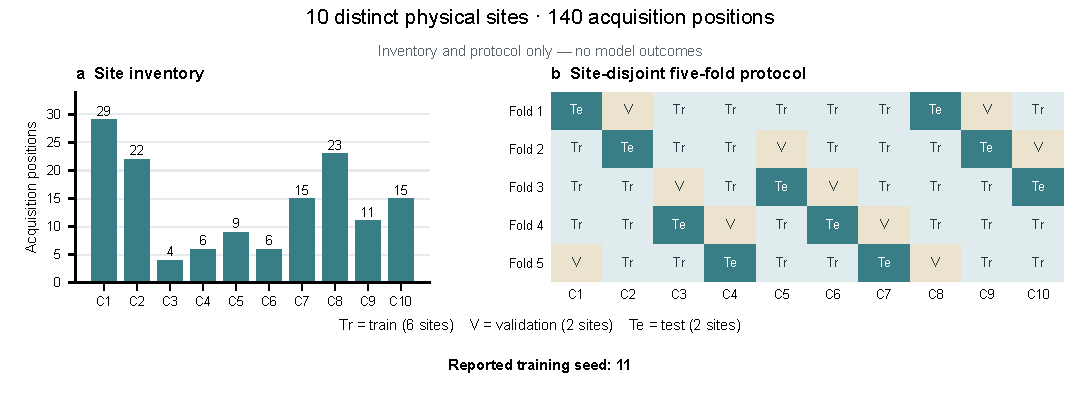
\includegraphics[width=\textwidth]{v3_inventory_folds.pdf}\caption{Acquisition scale and five-fold protocol.}\label{fig:inventory-folds}
\vspace{1pt}{\footnotesize\noindent Left: raw-view counts from acquisition metadata. Right: fixed training (Tr), validation (V) and test (Te) assignments.\par}\end{figure}

\section{Technical Validation}\label{sec:tech-en}
\subsection{Scope and evidence status}
Technical validation characterizes internal geometric consistency, the effects of input bands and controlled misalignment on colorization, and performance on held-out sites. The model results are an exploratory, resource-limited benchmark: single seed 11, provisional common support that has not passed human quality screening, and fixed last-step checkpoints. They are adaptations under this protocol, not faithful reproductions or evidence of convergence. Validation describes what the resource can currently measure rather than establishing a general ranking of models \cite{dodge2019,pineau2021}.

Two properties bound this evidence. Automatic pipeline diagnostics and controlled-misalignment responses do not independently measure registration accuracy. The model results use one support fixed across the current comparisons (\SupportPixelCount{} valid pixels, \QualifiedWindowCount{} qualified windows), but it has not been frozen after human acceptance. A change confined to evaluation masks can permit rescoring of retained predictions, subject to metric-specific support requirements. Changes to training inputs, loss support or splits require assessment of which models must be retrained; the present numbers cannot simply be relabelled under a changed protocol.

\subsection{Per-site support and digital-number coverage}
The ten output canvases contain 133,736,176 pixels, of which 88,861,466 (66.45\%) belong to the common support; this is not the full canvas area. Table~\ref{tab:support-en} separates SSIM centres from LPIPS coverage: 58,532,167 centres satisfy the complete $11\times11$ neighbourhood condition, while the union of 1,541 LPIPS rectangles contains 23,805,940 pixels, or 26.79\% of common support. Overlapping rectangles within a site count once in covered area. LPIPS covers only 1.54\% of common support at C1 but 82.74\% at C8. Equal-site perceptual scores therefore still describe eligible subregions with different sizes and content; they do not measure full-image perceptual quality.
\begin{table}[htbp]\centering
\caption{Per-site evaluation support for the reported metrics.}\label{tab:support-en}
\begingroup\footnotesize\setlength{\tabcolsep}{3pt}% Generated by make_support_statistics_20261015.py; counts use saved support.
\begin{tabular*}{\textwidth}{@{\extracolsep{\fill}}lrrrrrrr@{}}
\toprule
Site & \shortstack{Common\\Mpx} & \shortstack{Canvas\\(\%)} & \shortstack{SSIM centres\\million} & Windows & \shortstack{LPIPS\\rectangles} & \shortstack{Unique area\\Mpx} & \shortstack{Area/common\\(\%)} \\
\midrule
C1 & 10.653 & 48.97 & 5.153 & 754 & 10 & 0.164 & 1.54 \\
C2 & 13.189 & 77.49 & 7.243 & 936 & 67 & 0.991 & 7.52 \\
C3 & 6.224 & 91.87 & 4.909 & 396 & 214 & 3.257 & 52.34 \\
C4 & 5.837 & 94.02 & 5.406 & 339 & 275 & 4.355 & 74.62 \\
C5 & 9.463 & 71.67 & 5.379 & 678 & 17 & 0.279 & 2.94 \\
C6 & 4.650 & 56.33 & 3.675 & 303 & 88 & 1.435 & 30.85 \\
C7 & 10.479 & 61.05 & 6.730 & 697 & 32 & 0.520 & 4.96 \\
C8 & 12.361 & 64.08 & 12.006 & 770 & 670 & 10.228 & 82.74 \\
C9 & 7.775 & 61.99 & 4.116 & 494 & 135 & 2.108 & 27.11 \\
C10 & 8.231 & 71.44 & 3.915 & 526 & 33 & 0.469 & 5.70 \\
\midrule
Total & 88.861 & 66.45 & 58.532 & 5893 & 1541 & 23.806 & 26.79 \\
\bottomrule
\end{tabular*}
\endgroup
\vspace{2pt}{\footnotesize\noindent Common-support percentages use each output canvas as denominator. SSIM centres follow erosion of the common mask by an $11\times11$ all-one structure with a zero border. Unique LPIPS area is the union of saved $128\times128$ rectangles; its percentage uses common valid pixels as denominator. Total percentages use summed counts. Windows are current training candidates, not human-accepted samples.\par}
\end{table}

The existing geometry/privacy layer is saved as one combined mask. Within the cropped canvases it excludes 302,985 pixels only at C10 (2.630\% of that canvas). No pixels are excluded by that saved layer at the other sites; this does not establish the absence of local mismatch, motion or other quality defects. Within the retained geometry/privacy domain, the joint six-modality rule $0<\mathrm{DN}<250$ excludes a further 44,571,725 pixels (33.40\%). Appendix Tables~\ref{tab:exclusions-en}--\ref{tab:dynamic-en} report the site breakdown and per-modality threshold counts. These describe processed eight-bit images, not sensor saturation rates. An independently accepted human quality-exclusion layer is not yet available and must not be represented as zero exclusions.

\subsection{Registration quality from automatic diagnostics}
All ten scenes passed the automatic mosaic acceptance, covering cross-modal match counts, held-out residuals, corner deviation and intra-band consistency. Cross-modal (RGB against B1) held-out residual P95 spans 0.77--1.92 preview-grid pixels; the maximum within-SWIR residual P95 spans 3.48--6.25 output-grid pixels across scenes. These quantities use different grids and must not be compared directly or converted using the output scale alone. The values are internal consistency diagnostics of feature matching, not independent registration or geolocation accuracy. The output grid is scaled by \DatasetOutputScale{} relative to the B1 reference canvas; this convention does not specify a local conversion to sensor-native pixels. Per-scene diagnostics are included in the planned release.

\subsection{Colorization benchmark and non-neural references}
Table~\ref{tab:baseline-en} reports the main comparisons of four models and two non-neural references under equal-site averaging. The learned conditions require \TrainRunCount{} training runs in total. All conditions use the same test support (\SupportPixelCount{} common valid pixels), so the band ablation does not change which pixels are scored. For each fold, the linear reference samples input and RGB pixels on a grid with a 16-pixel stride in both axes inside the common valid support of the training sites. Samples are pooled across training sites to fit an affine map, including an intercept, from the selected bands to RGB by least squares; predictions are clipped to $[0,1]$. The channel reference maps normalized B1, B2 and B3 directly to R, G and B without fitting. Although recorded in the five-band run, it ignores B4 and B5. This definition matches the source code bound to all 15 saved reference records.

\begin{table}[htbp]
\centering
\caption{SWIR-to-RGB colorization, site-equal.}
\label{tab:baseline-en}
\vspace{1pt}{\footnotesize\noindent Single seed 11, fixed last-step checkpoints, provisional common support. Only the linear reference is fitted by least squares on training sites; the channel reference is unfitted.\par}
\small
\begin{tabular}{@{}lrrrrr@{}}
\toprule
Condition & PSNR/dB$\uparrow$ & SSIM$\uparrow$ & LPIPS$\downarrow$ & $\Delta E_{00}\downarrow$ & MAE$\downarrow$\\
\midrule
Linear reference (5 bands) & \PsnrLinearFive & \SsimLinearFive & \LpipsLinearFive & \DeltaELinearFive & 0.1602\\
Restormer (5 bands) & \PsnrRestormerFive & \SsimRestormerFive & \LpipsRestormerFive & \DeltaERestormerFive & 0.1559\\
TFD-GAN (5 bands) & \PsnrTfdFive & 0.4770 & 0.5517 & 22.2318 & 0.1782\\
U-Net (5 bands) & \PsnrUnetFive & 0.5259 & 0.5760 & 22.4280 & 0.1794\\
pix2pix (5 bands) & \PsnrPixFive & 0.4584 & 0.5554 & 22.4749 & 0.1801\\
pix2pix (B1, B2, B4) & \PsnrPixBOneTwoFour & 0.4704 & 0.5687 & 23.1051 & 0.1704\\
pix2pix (B1 only) & \PsnrPixBOne & \SsimPixBOne & 0.5591 & 24.2332 & 0.1678\\
B1/B2/B3 channel map & \PsnrChannelFive & 0.4979 & 0.6307 & 29.9596 & 0.2608\\
\bottomrule
\end{tabular}
\end{table}

Restormer has the highest site-equal PSNR among the learned models (\PsnrRestormerFive\,dB). Its difference from the linear reference (\PsnrLinearFive\,dB) is $-0.3122$\,dB, with a 95\% paired bootstrap interval of $[-1.5404,\,0.6467]$\,dB. The U-Net interval also crosses zero. The TFD-GAN and pix2pix intervals lie below zero: $[-2.4269,\,-0.2433]$ and $[-3.0685,\,-0.1991]$\,dB, respectively. Thus the learned models show no PSNR advantage over the linear reference under the current protocol, while the uncertainty differs by model. These and the band-comparison intervals use 10,000 paired bootstrap resamples of the ten sites (resampling seed 20261005), without correction for multiple comparisons. Training sets overlap across folds, so the five folds are not independent experimental replicates. The intervals are descriptive for these ten sites and this training seed and do not establish population-wide statistical conclusions. The following window-level comparison provides an additional, limited diagnostic.
\begin{figure}[htbp]\centering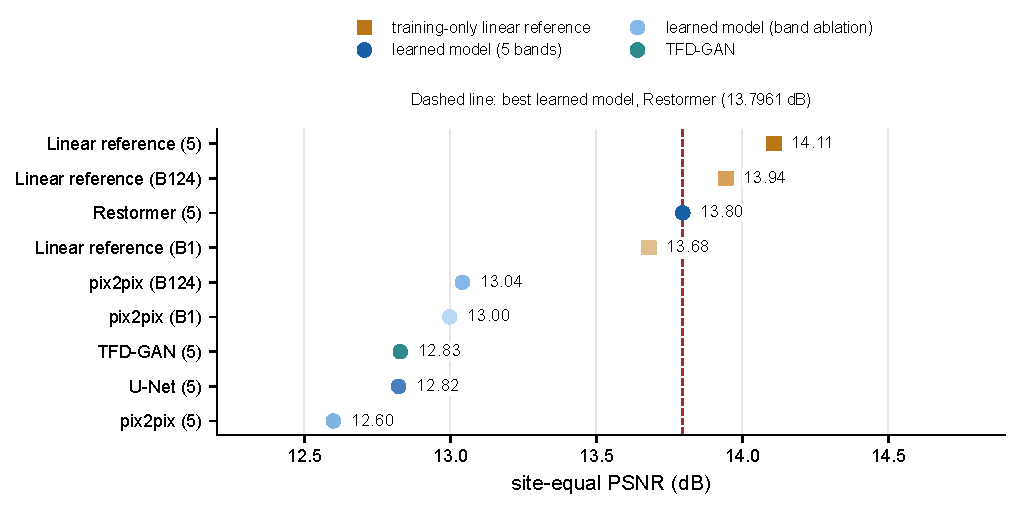
\includegraphics[width=\textwidth]{figV10_baseline_comparison.pdf}\caption{Site-equal PSNR for nine conditions.}\label{fig:baseline-en}
\vspace{1pt}{\footnotesize\noindent The figure shows six learned conditions and linear references with five bands, B1 and B1/B2/B4. The dashed line marks five-band Restormer (\PsnrRestormerFive\,dB), the highest PSNR among the learned models. Conditions share one test support; the learned conditions comprise \TrainRunCount{} training runs.\par}\end{figure}

\subsection{First-fold window diagnostic on training and held-out sites}
The first-fold pix2pix last-step checkpoint was evaluated without retraining on a fixed diagnostic set of training- and held-out-site windows. This set uses $256\times256$ windows with at least 90\% valid pixels and at most 48 windows per site, distinct from the main training-window rule and whole-scene benchmark. PSNR is first averaged across windows within each site, then equally across the included sites. Three training sites contribute \SeenWindowCount{} windows and average \SeenPsnr\,dB; two held-out sites contribute \HeldoutWindowCount{} windows and average \HeldoutPsnr\,dB, a \GeneralizationGap\,dB gap (Table~\ref{tab:generalization-en}). This comparison does not include all training sites, folds or models.

\begin{table}[htbp]
\centering
\caption{First-fold pix2pix diagnostic on selected training- and held-out-site windows.}
\label{tab:generalization-en}
\vspace{1pt}{\footnotesize\noindent The saved checkpoint is unchanged. Window PSNR is averaged within sites, then sites are weighted equally. B1 grayscale replication is scored on the same diagnostic windows and support; it has no learned weights.\par}
\small
\begin{tabular}{@{}llrrr@{}}
\toprule
Group & Sites (windows) & Windows & PSNR/dB$\uparrow$ & B1 gray copy/dB\\
\midrule
Training sites & C3(34), C4(42), C10(13) & \SeenWindowCount & \SeenPsnr & 12.34\\
Held-out sites & C1(1), C8(42) & \HeldoutWindowCount & \HeldoutPsnr & 11.79\\
\midrule
Gap & \multicolumn{2}{r}{training minus held-out} & \GeneralizationGap & 0.55\\
\bottomrule
\end{tabular}
\end{table}

Replicating B1 into three grayscale channels provides a simple diagnostic reference on the same windows and evaluation support. It is neither an information upper bound nor a calibrated measure of the information in that band. The model exceeds this reference by 13.04\,dB on the selected training sites (\SeenPsnr{} versus 12.34\,dB) and 1.80\,dB on the held-out sites (\HeldoutPsnr{} versus 11.79\,dB); gains are calculated at the saved precision before rounding. This demonstrates substantial fitting on the selected training windows and a much smaller advantage on the selected held-out windows. It is consistent with limited transfer under this setting, but does not isolate its cause or exclude optimization budget, model adaptation, support selection and site-content differences as contributing factors.

The five-fold whole-scene benchmark also varies by site: pix2pix with five bands spans 11.30--14.26\,dB. That benchmark uses different support from the window diagnostic above. The diagnostic draws on one fold and one seed with unbalanced window counts (C1 contributes only one window), and the run directory contains no stepwise validation sequence from which to establish convergence. The \GeneralizationGap\,dB difference is therefore limited evidence for these selected sites and windows, not a generalization-gap estimate for all 30 runs or a causal explanation of the whole-scene results \cite{roberts2017}.
\begin{figure}[htbp]\centering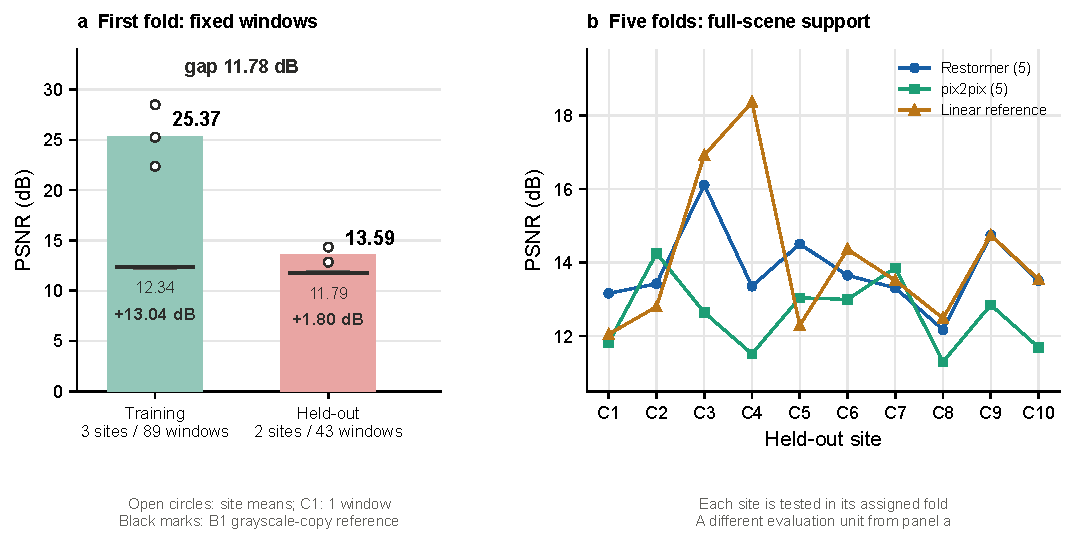
\includegraphics[width=\textwidth]{figV9_generalization_gap.pdf}\caption{First-fold window diagnostic and five-fold whole-scene variation.}\label{fig:generalization-en}
\vspace{1pt}{\footnotesize\noindent Left: first-fold pix2pix on three training sites (89 windows) and two held-out sites (43 windows, including one at C1); window PSNR is averaged within sites, then equally across sites. Open markers show site means; horizontal bars show B1 grayscale replication and labels show gains calculated before rounding. Right: five-fold whole-scene PSNR for three conditions across ten held-out sites. The two panels use different evaluation support. No model was retrained for the window diagnostic.\par}\end{figure}

\subsection{Band count and input configuration}
Three pix2pix input configurations share one test support: B1, B1/B2/B4 and all five bands. Relative to B1, five bands reduce \dE{} by 1.7584 (95\% paired interval for B1 minus five bands: $[0.5132,\,2.9355]$), while SSIM falls by 0.0430 (five bands minus B1: $[-0.0750,\,-0.0151]$). PSNR falls by about 0.40\,dB, but its paired interval crosses zero, as does the LPIPS interval. For five bands versus B1/B2/B4, the intervals for PSNR, SSIM, LPIPS and \dE{} all cross zero. The result is a trade-off between displayed-colour discrepancy and structural similarity, rather than evidence that every metric is unchanged or that five bands give a uniform benefit. These descriptive comparisons are limited to one model, one training seed and provisional support, with no multiple-comparison correction. Nominal passbands and the unmeasured system response also constrain interpretation in terms of material properties.

\subsection{Controlled misalignment}
Known displacements were applied to the saved five-fold pix2pix models. Displacements are defined on the B1 reference mosaic grid at 0, 0.5, 1, 2 and 4\,pixels, retaining four directions and perturbing either all SWIR bands or B1 alone, yielding \SensitivityRecordCount{} site-level records. Table~\ref{tab:sensitivity-en} reports loss relative to zero displacement: PSNR loss is baseline minus perturbed PSNR, and colour-error increase is perturbed minus baseline \dE{}. At 4\,pixels, joint perturbation lowers site-equal PSNR by 0.4451\,dB and raises \dE{} by 0.8212. Perturbing B1 alone produces roughly half the PSNR loss (0.2112\,dB), but a similar colour-error increase (0.7877). Loss generally increases with displacement; the B1-only 0.5-pixel condition slightly improves PSNR, so the response is not strictly monotonic from zero.

\begin{table}[htbp]
\centering\small
\caption{Performance loss under controlled misalignment.}\label{tab:sensitivity-en}
\vspace{1pt}{\footnotesize\noindent Positive values denote deterioration relative to zero displacement. Displacements use the B1 reference grid; four directions are retained.\par}
\begin{tabular}{@{}lrrrr@{}}
\toprule
Displacement/pixels & \multicolumn{2}{c}{All SWIR bands} & \multicolumn{2}{c}{B1 only}\\
& PSNR loss/dB & \dE{} increase & PSNR loss/dB & \dE{} increase\\
\midrule
0.5 & 0.0144 & 0.0270 & $-0.0040$ & 0.0131\\
1.0 & 0.0581 & 0.1144 & 0.0048 & 0.0757\\
2.0 & 0.1836 & 0.3425 & 0.0569 & 0.2983\\
4.0 & 0.4451 & 0.8212 & 0.2112 & 0.7877\\
\bottomrule
\end{tabular}
\end{table}

This measures algorithmic response to a known displacement, not independent sensor-frame registration accuracy, and does not substitute for human geometric validation.
\begin{figure}[htbp]\centering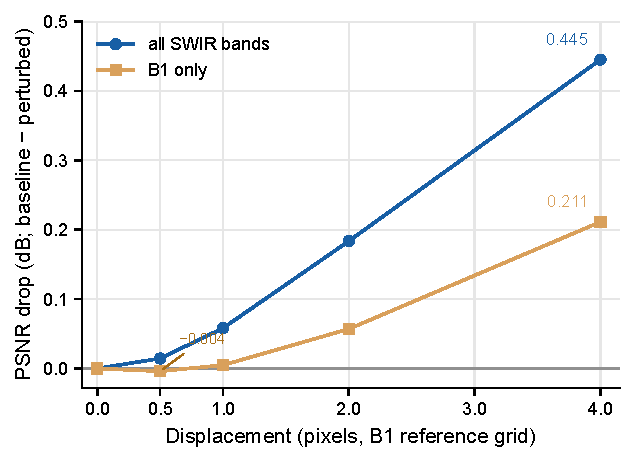
\includegraphics[width=0.52\textwidth]{figV11_misalignment_sensitivity.pdf}\caption{PSNR loss under controlled misalignment.}\label{fig:sensitivity-en}
\vspace{1pt}{\footnotesize\noindent Site-equal PSNR loss is zero-displacement PSNR minus perturbed PSNR; a negative value denotes improvement. All SWIR bands are perturbed together or B1 alone. This is not a measure of independent registration accuracy.\par}\end{figure}

\subsection{Dependence on the aggregation convention}
The main analysis retains the existing equal-site aggregation convention. Under pixel-pooled mean squared error converted to PSNR, Restormer (\PooledPsnrRestormer\,dB) slightly exceeds the linear reference (\PooledPsnrLinear\,dB), reversing the site-equal ordering. The two estimands differ: equal-site averaging describes the average site, whereas pixel pooling weights sites by valid-pixel count. Both conventions are reported, with equal-site averaging used consistently for the main comparisons. This sensitivity does not establish overall superiority of either method, and the manuscript does not claim that the analysis was preregistered.
\begin{figure}[htbp]\centering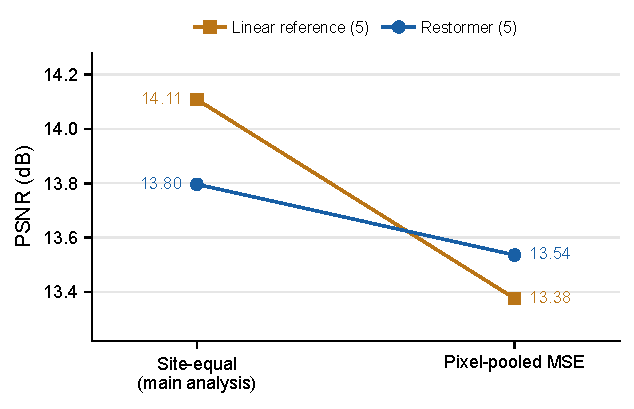
\includegraphics[width=0.48\textwidth]{figV12_aggregation.pdf}\caption{Ordering under two aggregation conventions.}\label{fig:aggregation-en}\end{figure}

\subsection{Visual inspection}
The existing retrospective visual inspection saved two fixed windows per site, twenty in total. Window A maximizes common valid-pixel count, then minimizes distance to the canvas centre, with coordinates breaking ties. Window B excludes candidates overlapping A and uses the same valid-pixel priority near a fixed upper-right quarter point. Coordinates were saved before predictions were loaded in that inspection; this does not establish experiment preregistration. Figures~\ref{fig:local-modalities-en} and~\ref{fig:local-predictions-en} take A windows from every third site in numerical order (C1, C4, C7 and C10), a deterministic illustrative subset selected without model scores or visual ranking. All four windows have 100\% common support. The Supplementary Visual Atlas retains all twenty windows and six learned conditions, identified by site, window and top-left coordinates.

In the displayed windows, the C1 window-frame structure is partly retained but predictions shift towards blue; predictions of the road surface at C4 shift towards green. Regular texture is visible in the pix2pix outputs at C7 and C10, and the C10 predictions differ in colour from the dark-blue RGB target. These observations describe the displayed windows only: they do not estimate defect prevalence or attribute causes to registration or a model component. The six-modality crops show same-coordinate content and do not replace independent geometric validation. This machine-assisted inspection is recorded separately from human quality acceptance.
\begin{figure}[p]\centering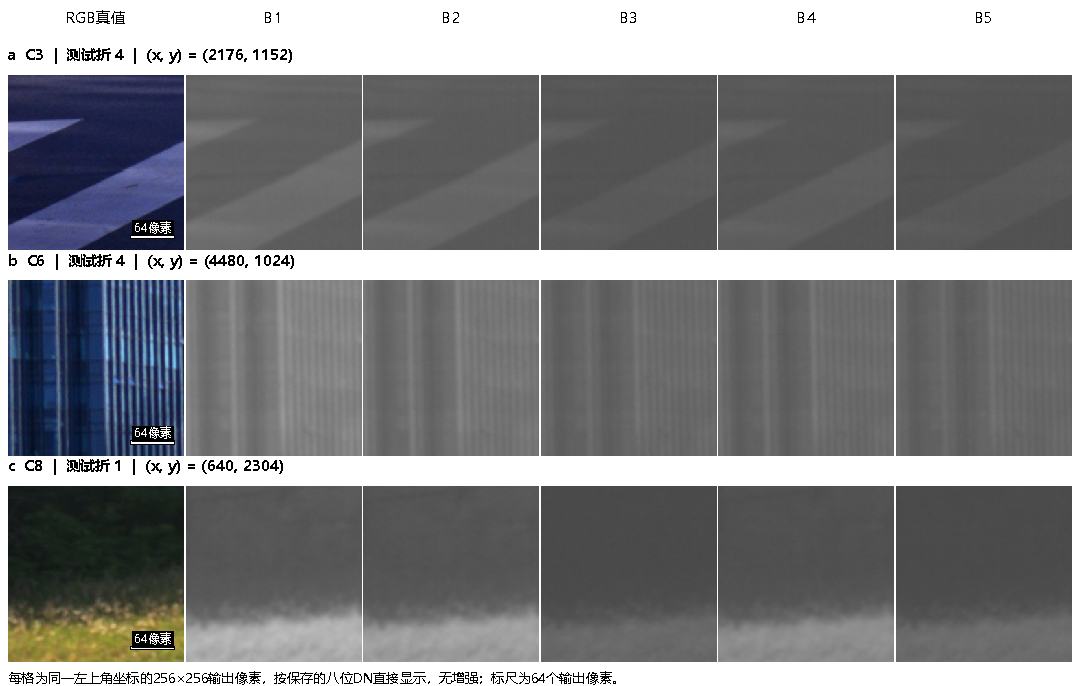
\includegraphics[width=\textwidth]{fig_local_modalities_20261015.pdf}
\caption{Six-modality local views at fixed windows.}\label{fig:local-modalities-en}
\vspace{2pt}{\footnotesize\noindent Each panel shows $256\times256$ output pixels from the same top-left coordinate. Bars denote 64 output pixels, not a physical distance or calibrated native-sensor scale. RGB and B1--B5 use saved eight-bit DN directly, without per-image contrast stretching or sharpening. Row labels give site, window, test fold and coordinates. Shared output coordinates do not establish independently validated alignment.\par}\end{figure}
\begin{figure}[p]\centering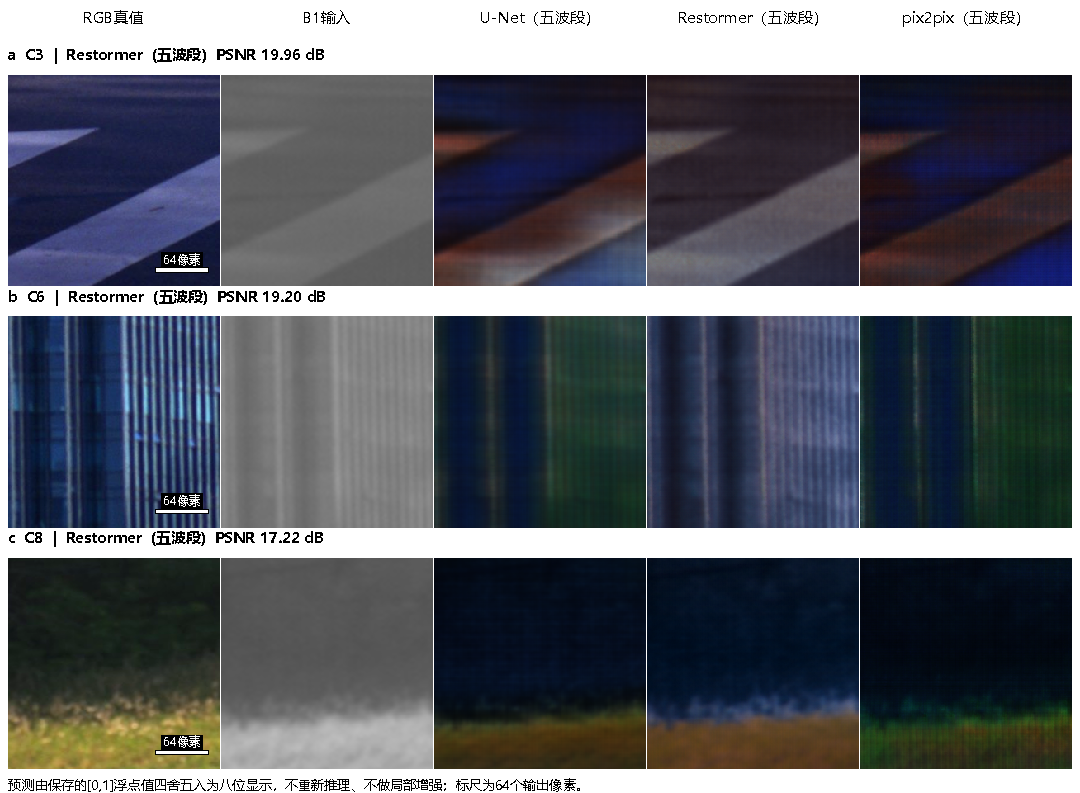
\includegraphics[width=\textwidth]{fig_local_predictions_20261015.pdf}
\caption{Inputs, RGB targets and saved predictions at the same fixed windows.}\label{fig:local-predictions-en}
\vspace{2pt}{\footnotesize\noindent All three models use five input bands and seed 11; predictions come from each site's assigned held-out fold. B1 illustrates one input band only. Saved floating-point predictions in $[0,1]$ are rounded to eight-bit display without new inference or local enhancement. Windows match the six-modality plate; bars denote 64 output pixels. The Supplementary Visual Atlas includes all twenty windows and six learned conditions. These views do not establish an overall model ranking.\par}\end{figure}

\subsection{Pools, splitting and training protocol}
Training windows are $256\times256$ with stride 128 and an appended final start. The current geometry and privacy masks must be valid throughout a window, and at least 50\% of pixels must lie in the common six-modality dynamic-range support ($0<\mathrm{DN}<250$). These mask conditions do not imply completed human quality or privacy acceptance. The same support is used across input-band conditions. Pixel reconstruction uses valid pixels; gradient terms require two valid adjacent pixels. GAN, VGG-feature and low-pass colour paths use a common neutral fill outside support; these are not pixel-masked perceptual losses. The current experiments use the common pool without human quality screening. EX-4 comparisons between quality pools are outside this manuscript's scope.

\begin{table}[htbp]\centering\small
\caption{Site-disjoint five-fold assignment.}\label{tab:protocol}
\begin{center}\footnotesize\noindent Each site appears in a test pair once; all folds use training seed 11.\end{center}
\begin{tabular}{clll}\toprule Fold & Training sites & Validation sites & Test sites\\\midrule
1 & C3,C4,C5,C6,C7,C10 & C2,C9 & C1,C8\\
2 & C1,C3,C4,C6,C7,C8 & C5,C10 & C2,C9\\
3 & C1,C2,C4,C7,C8,C9 & C3,C6 & C5,C10\\
4 & C1,C2,C5,C8,C9,C10 & C4,C7 & C3,C6\\
5 & C2,C3,C5,C6,C9,C10 & C1,C8 & C4,C7\\\bottomrule\end{tabular}\end{table}

The models are U-Net \cite{ronneberger2015unet}, pix2pix \cite{isola2017,goodfellow2014gan,mirza2014cgan}, TFD-GAN \cite{chen2026thesis} and Restormer \cite{zamir2022restormer}. Current budgets are respectively 20k, 20k, 12k and 40k updates with batch sizes 8, 8, 8 and 2. Neither sample exposure nor compute is equalized; this is a resource-limited practical benchmark. AdamW uses a constant learning rate of $2\times10^{-4}$ and the last-update model, without early stopping or test-based checkpoint selection \cite{cawley2010}. The configuration selects sixteen distinct windows per validation site for monitoring; the main benchmark evaluates whole scenes. Digital numbers are mapped to $[0,1]$ for Restormer and $[-1,1]$ otherwise. All reported training runs use seed 11 and are aggregated equally across sites. A single training seed cannot estimate seed variance; the site-level intervals describe these limited sites rather than guaranteeing population generalization \cite{roberts2017}.

\subsection{Full-scene evaluation and metric supports}
All compared conditions use the same current test support, fixed for this comparison but not frozen after human acceptance. Predictions are assembled in floating point and clipped consistently to $[0,1]$ before scoring. Metric supports differ where their definitions require neighbourhoods or rectangles, and each support is reported separately.
\begin{table}[htbp]\centering\small
\caption{Metric definitions and evaluation supports.}\label{tab:metrics}
\vspace{1pt}{\footnotesize\noindent These are protocol definitions, not measured results.\par}
\begin{tabularx}{\textwidth}{p{0.18\textwidth}X}\toprule Metric & Definition and support\\\midrule
PSNR / MAE / RMSE \cite{huynhthu2008} & Whole-scene valid paired pixels on $[0,1]$ RGB; report common pixel support.\\
SSIM \cite{wang2004} & $11\times11$ Gaussian window, $\sigma=1.5$; centres require a completely valid neighbourhood.\\
$\Delta E_{00}$ \cite{luo2001ciede2000,sharma2005} & sRGB conversion with D65/2$^\circ$; mean, median and P95 on valid pixels. This is displayed-colour discrepancy, not reflectance accuracy.\\
LPIPS \cite{zhang2018lpips} & LPIPS-Alex v0.1 on shared rectangles lying entirely inside the dynamic-range usability layer. Validity cannot be masked inside a perceptual rectangle, so the side is set to 128: at 256 two sites admit no rectangle under this validity rule, whereas 128 admits rectangles at every site and exceeds the implementation's 64-pixel floor. Rectangle scores are reported separately from the per-site rectangle counts and unique covered areas in Table~\ref{tab:support-en}. This does not measure full-image perceptual performance.\\\bottomrule\end{tabularx}\end{table}

\subsection{Factorial scope and reuse controls}
The current scope comprises EX-0 data statistics, EX-1 four models across five folds with one training seed (20 runs), EX-2 pix2pix B1/B124 ablations (10 additional runs, reusing EX-1 five-band runs), and EX-3 inference-offset sensitivity using retained models. B1 and B124 are controlled input configurations within this dataset; narrowband B1 does not reproduce an external broadband SWIR sensor. Resource-attribute positioning is not cross-dataset numerical superiority \cite{jin2026,brown2011}.

EX-3 uses pix2pix with offsets of 0, 0.5, 1, 2 and 4 pixels on the B1 reference mosaic grid, retaining four directions and perturbing all SWIR bands or B1 alone. Five folds require 165 fold--condition evaluations (330 site evaluations), with the zero-offset case recomputed on common support. This measures response to known shifts, not independent sensor-frame registration accuracy. EX-4 three-pool comparisons are outside this manuscript's scope. If only evaluation masks change, retained predictions may be rescored on the revised support; changes to training images, loss support or splits require a separate retraining assessment.

\section{User Notes and limitations}
Ten distinct sites support site-disjoint reuse, but the dataset is small and not an environmentally representative sample. Whole-scene pix2pix PSNR with five bands ranges from 11.30 to 14.26\,dB across sites; reusers should report site variation and consider dependence. Nominal passbands, sequential exposures, uncalibrated digital numbers and resampling constrain spectral and spatial interpretation. Inter-band pixel ratios are not reflectance ratios, and geometric fitting cannot remove motion caused by sequential acquisition.

The model results use one training seed and provisional common support, so seed variance is not estimated. The first-fold window diagnostic is limited to three training sites and two held-out sites, and does not establish the cause of the observed gap. Negative results, failure cases and aggregation sensitivity are retained \cite{dodge2019}.

Three details matter for reuse. Geometry, privacy and dynamic-range conditions jointly define the evaluated pixels. LPIPS is evaluated only on fully valid $128\times128$ rectangles shared across conditions, with substantially different counts across sites; it is not full-image perceptual performance. Equal-site and pixel-pooled aggregation give different orderings here, so their conventions must be checked before comparing studies. Formal human geometric validation, quality acceptance and public reproduction remain distinct from the current automatic diagnostics and local model evaluation.

\section*{Code Availability}
The local project contains mosaicking and registration, mask and support construction, four-model training drivers, sensitivity inference, metrics and checks. Local run records track data and support identities, source hashes and library versions. A public code URL, fixed release commit, dependencies, licence terms and an independent minimal reproduction check remain to be finalized. The intended code release will provide the records needed to recompute the reported quantities on the corresponding support.
\section*{Data Availability Statement}
The dataset is intended for Zenodo under a proposed CC BY 4.0 licence, subject to confirmation of rights and release scope. The planned package comprises 60 output TIFFs with SHA-256 bindings, the selected source-frame set, scene transforms and crop records, source and acquisition evidence, masks and window lists, evaluation-support records and privacy-redaction layers. A public URL, release identifier, DOI, dataset citation, review link and download/hash verification remain pending. Physical-site identity is based on author confirmation rather than independent external verification; acquisition dates retain their stated evidence, including the author correction for C8 and the previous file-time inference. C10 has seven identified licence-plate regions, but their redaction does not establish that all images are free of identifiable faces or plates. Full privacy review of source imagery, mosaics, previews and annotation products remains incomplete and is required before public release. Reusers should also cite the related earlier same-platform work.

\section*{Acknowledgements}
The authors thank Qidong Chen for participating in the original data acquisition, for authorising the use of his TFD-GAN implementation in the model-family comparison, and for the acquisition-platform description and band-selection rationale cited in the Methods. Each acknowledged individual has consented to being named.
\section*{Author Contributions}
H.D.: conceptualization, data curation, formal analysis, investigation, methodology, software, validation, visualization, and writing--original draft. X.L.: conceptualization, methodology, project administration, resources, supervision, validation, and writing--review \& editing. L.D.: data curation, investigation, resources, validation, and writing--review \& editing. C.H.: data curation.

\section*{Funding}
No additional funding was received specifically for the preparation of this Data Descriptor.

\section*{Conflicts of Interest}
The authors declare no competing interests.

\bibliographystyle{unsrtnat}
\bibliography{refs}
\clearpage
\appendix
\section{Support layers and digital-number threshold counts}
These statistics use the same saved mosaics and masks; they describe current evaluation support without constituting new human quality acceptance. Canvas refers to the output after common-coverage cropping and cannot quantify the fraction removed from the original acquisition fields of view.
\begin{table}[htbp]\centering\small
\caption{Exclusion fractions from the saved combined mask and joint dynamic-range rule.}\label{tab:exclusions-en}
% Geometry/privacy is a combined existing layer; no human quality layer exists.
\begin{tabular*}{\textwidth}{@{\extracolsep{\fill}}lrr@{}}
\toprule
Site & \shortstack{Geometry/privacy excluded\\of canvas (\%)} & \shortstack{Joint DN excluded\\of geometry/privacy domain (\%)} \\
\midrule
C1 & 0.000 & 51.03 \\
C2 & 0.000 & 22.51 \\
C3 & 0.000 & 8.13 \\
C4 & 0.000 & 5.98 \\
C5 & 0.000 & 28.33 \\
C6 & 0.000 & 43.67 \\
C7 & 0.000 & 38.95 \\
C8 & 0.000 & 35.92 \\
C9 & 0.000 & 38.01 \\
C10 & 2.630 & 26.63 \\
\midrule
Total & 0.227 & 33.40 \\
\bottomrule
\end{tabular*}

\vspace{2pt}{\footnotesize\noindent The first percentage uses the output canvas as denominator; the second uses the retained geometry/privacy domain, so the percentages cannot be added. Existing files do not separate geometric and privacy causes or provide an accepted human quality layer.\par}\end{table}
\begin{table}[htbp]\centering\footnotesize
\caption{Per-site and per-modality digital-number threshold fractions.}\label{tab:dynamic-en}
% Each cell = percent zero / percent >= 250, denominator geometry/privacy pixels.
\begin{tabular*}{\textwidth}{@{\extracolsep{\fill}}lrrrrrr@{}}
\toprule
Site & RGB & B1 & B2 & B3 & B4 & B5 \\
\midrule
C1 & 3.35/40.72 & 0.00/16.23 & 0.00/8.38 & 0.00/0.23 & 0.00/2.55 & 0.00/0.12 \\
C2 & 13.44/9.44 & 0.00/0.10 & 0.00/0.05 & 0.00/0.06 & 0.00/0.04 & 0.00/0.05 \\
C3 & 5.53/2.49 & 0.00/0.72 & 0.00/0.19 & 0.00/0.01 & 0.00/0.01 & 0.00/0.01 \\
C4 & 1.13/1.75 & 0.00/3.52 & 0.00/0.38 & 0.00/0.00 & 0.00/0.00 & 0.00/0.00 \\
C5 & 3.10/14.48 & 0.00/17.01 & 0.00/0.19 & 0.00/0.03 & 0.00/0.02 & 0.00/0.02 \\
C6 & 0.68/41.08 & 0.00/6.72 & 0.00/2.42 & 0.00/0.00 & 0.00/0.03 & 0.00/0.00 \\
C7 & 0.90/31.79 & 0.00/10.10 & 0.00/2.64 & 0.00/0.05 & 0.00/0.18 & 0.00/0.01 \\
C8 & 0.00/35.92 & 0.00/0.00 & 0.00/0.00 & 0.00/0.00 & 0.00/0.00 & 0.00/0.00 \\
C9 & 26.10/11.89 & 0.00/0.04 & 0.00/0.00 & 0.00/0.00 & 0.00/0.00 & 0.00/0.00 \\
C10 & 10.23/15.89 & 0.00/4.75 & 0.00/2.59 & 0.00/1.11 & 0.00/1.65 & 0.00/1.06 \\
\bottomrule
\end{tabular*}

\vspace{2pt}{\footnotesize\noindent Each cell gives the percentage at DN=0 followed by the percentage at DN$\geq250$, with retained geometry/privacy pixels as denominator. RGB meets a condition when any channel does; conditions and modalities can overlap and their percentages must not be summed. Values of 0.00 are rounded, not necessarily exact zero. These are not raw-sensor saturation rates or material reflectance measurements. Exact counts and source identities accompany the support statistics.\par}\end{table}
\end{document}
